\documentclass{llncs}

% name of the language
\newcommand{\lang}[0]{MediatE}

\title{A New Coordination Language \lang{}}

\author{Yi Li\and Meng Sun}
\institute{LMAM and Department of Informatics, School of Mathematical Sciences, Peking University, Beijing, China \\
\email{liyi\_math@pku.edu.cn, sunmeng@math.pku.edu.cn}
}


\usepackage{listings}
\usepackage{textcomp}
\usepackage{xcolor}
\usepackage{enumitem}
\usepackage{amssymb}
\usepackage{empheq}
\usepackage{mathpartir}
% \usepackage{pxfonts}
\usepackage{fancybox}
\usepackage{algorithmic}
\usepackage{algorithm}
\usepackage[normalem]{ulem}
\usepackage{tikz}

\makeatletter
\newenvironment{CenteredBox}{% 
\begin{Sbox}}{% Save the content in a box
\end{Sbox}\centerline{\parbox{\wd\@Sbox}{\TheSbox}}}% And output it centered
\makeatother

\newcommand{\liyi}[1]{\textcolor{red}{#1}}
\renewcommand{\ttdefault}{pxtt}

\newtheorem{formalization}{Formalization}

\lstdefinelanguage{newlang}{
    keywords = {
        automaton,
        system,
        type,
        in, out,
        variables, transitions, statements, components, connections, 
        interface, func,
        sync,
        internals,
        begin, end,
        return,
        init, as,
        int, bool, char, enum, real
    },
    alsodigit = {-}
}

\lstset{
    basicstyle=\small\ttfamily, 
    numbers=left,
    numberstyle=\scriptsize,
    columns=flexible,
    numbersep=10pt,
    tabsize=2,
    extendedchars=true,         %
    breaklines=true,
    keywordstyle=\bfseries,
    stringstyle=\color{white}\ttfamily, % Farbe der String
    xleftmargin=17pt,
    framexleftmargin=17pt,
    framexrightmargin=5pt,
    framexbottommargin=4pt,
    % backgroundcolor=\color{lightgray},
    showstringspaces=false,
    language=newlang
}

% terminal symbols
\newcommand{\tsym}[1]{\:\mbox{\texttt{#1}}\:}
% non-terminal symbols
\newcommand{\ntsym}[1]{\:\langle\mbox{\emph{#1}}\rangle\:}


\newcommand*\widefbox[1]{\fbox{\hspace{1em}#1\hspace{1em}}}

\newenvironment{bnf}{%
    % \vspace{-1em}
    \setkeys{EmphEqEnv}{align*}%
    \setkeys{EmphEqOpt}{box=\widefbox}%
    \EmphEqMainEnv%
}{
    \endEmphEqMainEnv
    % \vspace{-1em}
}

\newcommand{\subtype}[0]{\preccurlyeq}

\newcommand\T{\rule{0pt}{2.6ex}}       % Top strut
\newcommand\B{\rule[-1.2ex]{0pt}{0pt}} % Bottom strut

\newcommand\smalltitle[1]{
    \vspace{0.2cm}
    \noindent\emph{{#1}.}
}

\begin{document}

\maketitle

\begin{abstract}
tbd
\end{abstract}

\section{Introduction}

\section{Overview}

% \begin{figure}
%     \begin{bnf}
%         \ntsym{program} &::=& (\ntsym{typeDef}|\ntsym{funcDef}|\ntsym{automataDef}|\ntsym{systemDef})^* \\
%         \ntsym{typeDef} &::=& \tsym{typedef} \ntsym{type} \tsym{as} \ntsym{name} \\
%         \ntsym{funcDef} &::=& \tsym{function} \ntsym{template} \ntsym{name} \ntsym{interface} \ntsym{funcBody} \\
%     \end{bnf}
%     \caption{Abstract Syntax Tree}
% \end{figure}

The goal of this language \lang{} mainly focus on:

\begin{enumerate}
    \item Compositional Verification.
\end{enumerate}
\section{Syntax of \lang{}}
\label{sec:syntax}

\begin{bnf}
    \ntsym{program} ::=  (& \ntsym{import} | \ntsym{typedef} | \ntsym{function} \\
    |& \ntsym{automaton} | \ntsym{system})^*
\end{bnf}

In the following subsections, we are going to take a simple \emph{queue} as an example, to illustrate how certain language elements are used to compose a model.

\subsection{Type System}
\label{subsec:typesystem}
\lang{} provides a rich-featured type system that supports various commonly-used data types in both formal modeling languages and programming languages.

\vspace{0.3em}
\noindent\emph{Primitive Type.} Table. \ref{table:primitivetypes} shows the primitive types supported in \lang{}.

\begin{table}
    \caption{Primitive Data Types}
    \label{table:primitivetypes}
    \centering
    \begin{tabular}{lcr}
        \hline
        Name & Declaration & Term Example \T\B \\
        \hline
        \T Bounded Integer\hspace{0.5cm} & \texttt{int lowerBound .. upperBound}\hspace{0.5cm} & \texttt{-1,0,1} \\
        Integer & \texttt{int} & \texttt{-1,0,1} \\
        Real & \texttt{real} & \texttt{0.1, 1E-3} \\
        Boolean & \texttt{bool} & \texttt{true, false} \\
        Character & \texttt{char} & \texttt{'a', 'b'} \\
        \B Enumeration & \texttt{enum {item$_1$, ..., item$_n$}} & \texttt{enumname.item} \\
        \hline
    \end{tabular}
\end{table}

\noindent\emph{Composite Type.} Composite type offers an approach to contruct complex data types with simpler ones. Several composite patterns are introduced as follows,

\begin{table}
    \caption{Composite Data Types (\texttt{T} denotes an arbitrary data type)}
    \centering
    \begin{tabular}{lr}
        \hline
        Name & Declaration \T\B \\
        \hline
        \T Tuple  & \texttt{T$_1$,...,T$_n$ }\\
        Union & \texttt{T$_1$|...|T$_n$ } \\
        Array & \texttt{T [length]}\\
        Slice & \texttt{T []} \\
        Map & \texttt{map [T$_{key}$] T$_{value}$} \\
        Struct\hspace{1cm} & \texttt{struct \{ field$_1$:T$_1$,..., field$_n$:T$_n$ \}} \\
        \B Initialized & \texttt{T$_{base}$ init term} \\
        \hline
    \end{tabular}
\end{table}

\begin{itemize}
    \item \emph{Tuple}. The \emph{tuple} operator `,' can be used to construct a finite tuple type with several base types.
    \item \emph{Union}. The \emph{union} operator `$|$' is designed to combine \emph{disjoint} types as a more complicated one. This is similar to the union type in C language but much easier to use.
    \item \emph{Array} and \emph{Slice}. An \emph{array} $T[n]$ is a finite ordered collection containing exactly $n$ elements of type $T$. Moreover, a \emph{slice} is an array of which the capacity is not specified, i.e. slice is a dynamic array.
    \item \emph{Map}. A \emph{map }[$T_{key}$] $T_{val}$ is a dictionary that maps a key of type $T_{key}$ to a value of type $T_{val}$.
    \item \emph{Struct}. A \emph{struct }\{$field_1:T_1,\cdots,field_n:T_n$\} contain $n$ fields, each has a particular type $T_i$ and a unique identifier $id_i$.
    \item \emph{Initialized}. A initialized type make it able to specify default values to types.
\end{itemize}

For simplicity in formalizing data types, we introduce the concept \emph{domain} of a type. 

\begin{formalization}[Domain]
    We use $Dom(T)$ to denote the value domain of type $T$, i.e. the set of all possible value of $T$.
\end{formalization}

\begin{example}[Types Used in A Queue] Now let us introduce some type declarations and local variables used in an automaton \texttt{Queue}. As shown in the following code fragment, we declares a singleton enumeration \texttt{NULL}, which contains only one element \texttt{null}. The buffer of a queue is in turn formalized as an array of \texttt{T} or \texttt{NULL}, indicating that a queue element can be either an assigned item or empty. The head and tail pointer are defined as two bounded integers.
\begin{lstlisting}
typedef enum {null} init null as NULL;
automaton <T:type,size:int> Queue(A:in T, B:out T) {
    variables {
        buf : ((T | NULL) init null) [size];
        phead : int 0 .. (size - 1) init 0;
        ptail : int 0 .. (size - 1) init 0;
    }
    ...
}
\end{lstlisting}
\end{example}

\subsection{Functions}

The abstract syntax tree of functions is shown as follows.
\begin{bnf}
    \ntsym{funcDecl} ::= & \tsym{function} \ntsym{template}^? \ntsym{identifier} \tsym{(} \ntsym{arguments} \tsym{)} \tsym{\{} \\
    & (\tsym{variables} \tsym{\{} \ntsym{varDecl}^* \tsym{\}})^? \\
    & \tsym{statements} \tsym{\{} \ntsym{assignStmt}^* \ntsym{returnStmt} \tsym{\}} \\
    \ntsym{assignStmt} ::= & \ntsym{term} \tsym{:=} \ntsym{term} \\
    \ntsym{returnStmt} ::= & \tsym{return} \ntsym{term} \\
    \ntsym{varDecl} ::= & \ntsym{identifier} \tsym{:} \ntsym{type} (\tsym{init} \ntsym{term})^? 
\end{bnf}
Basically, definition of a function includes:
\begin{itemize}
    \item An optional template including a set of parameters. A parameter can be either a type parameter (decorated by \texttt{type}) or a value parameter (decorated by its type). All possible parameter values of a function should be located statically.
    % TODO: how?
    Parameters in the template can be used in all the following language elements, e.g. type of input variables and return value, local variables and function statements.
    \item An identifier that indicates the name of this function.
    \item A set of read-only input variables.
    \item A optional set of local variables.
    \item A list of ordered statements that describes how the return value is calculated. Such a list must be ended by a \texttt{return} statement.
\end{itemize}
Functions in \lang{} are side-effect free. In other words, only local variables are writable in its assignment statements.
\begin{example}[Incline Operation on a Queue Pointer] The simple function describes how pointers are inclined. When a pointer is going to exceed its upper bound (determined by the parameter \emph{size}), we will reset it to zero.
    \label{exp:successor_function}
    \begin{lstlisting}
function <size:int> next(pcurr:int 0..(size-1)) : int 0..(size-1) {
    statements { return (pcurr + 1) % size; }
}
    \end{lstlisting}
\end{example}

% TODO: a more complicated function

\subsection{Automata : The Basic Behavioral Unit}

\begin{bnf}
    \ntsym{automaton} ::=& \tsym{automaton}\ntsym{template}^?\ntsym{identifier} \tsym{(} \ntsym{port}^* \tsym{)} \tsym{\{}\\
    & (\tsym{variables} \tsym{\{} \ntsym{varDecl}^* \tsym{\}})^? \\
    & \tsym{transitions} \tsym{\{} \ntsym{transition}^* \tsym{\}} \tsym{\}} \\
    \ntsym{port} ::=& \ntsym{identifier} \tsym{:} (\tsym{in}|\tsym{out}) \ntsym{type} \\
    \ntsym{transition} ::=& \ntsym{guardedStmt} | \tsym{group} \tsym{\{} \ntsym{guardedStmt}^* \tsym{\}}\\
    \ntsym{guardedStmt} ::=& \ntsym{term} \tsym{->} (\ntsym{stmt} | \tsym{\{} \ntsym{stmt}^* \tsym{\}}) \\
    \ntsym{stmt} ::=& \ntsym{term} \tsym{:=} \ntsym{term} | \tsym{perform} \ntsym{identifier}^+
\end{bnf}

\vspace{0.2cm}
\noindent \emph{Template.} Very similar to functions, a automaton can also be decorated with a set of template parameters, either value parameters or type parameters.

\vspace{0.2cm}
\noindent \emph{Ports.} Each automaton contains a set of ports, either \texttt{in}-coming or \texttt{out}-going, to communicate with the environment. To ensure the well-defineness of automata, ports are required to have an \emph{initialized} type, e.g. \texttt{int 0..1 init 0} instead of \sout{\texttt{int 0..1}}.

\vspace{0.2cm}
\noindent \emph{Variables.} Two types of variables are used in a automaton definition, they are:
\begin{enumerate}
    \item \emph{Local variables} that are declared in the \emph{variables} section. A local variable can only be referenced in its scope, i.e. the automaton definition. And similar to the ports, only initialized types are permitted when declaring local variables.
    \item \emph{Adjoint variables} that are used to describe the status of ports. For a port A, we assume that it has two boolean fields \texttt{A.reqRead} and \texttt{A.reqWrite} indicating if there is a pending \emph{read} or \emph{write} request on this port, and a data field \texttt{A.value} indicating the current value of this port (if a write operation is performed, \texttt{A.value} will be reassigned).
\end{enumerate}

A reasonable rule comes up that, both the \texttt{reqWrite} field of a input port and the \texttt{reqRead} field of a output port are \emph{read-only}. Similarly, we cannot rewrite the \texttt{value} field of a input port.

\smalltitle{Transitions} Similar to the PRISM\cite{KwiatkowskaCav2011} language, behavior of a channel in \lang{} is described by a series of guarded transitions (groups). As shown in  Example \ref{exp:trans_queue}, a \emph{transition} comprises two parts: a boolean term \emph{guard} that shows on what condition the transition could be fired, and a (set of) statement(s) that describe what will happen if the transition is fired. Two types of statements are supported in automata,
\begin{itemize}
    \item \emph{Assignment Statements} (\texttt{var$_1$,...,var$_n$ := term$_1$,...,term$_n$}). Local variables and writable adjoint variables are permitted to be assigned here. We can also assign several variables at the same time (similar to the tuple assignment in Python).
    \item \emph{Perform Statements} (\texttt{perform port$_1$,...,port$_n$}). Informally speaking, perform statements tell the environment to fire data operations on the output ports, or wait until being noticed that data operation on the input ports are fired by the environment (other automata, actually). Consequently, it's reasonable to require that the value of an input port should never be referred until the port is performed. Similarly, the value of an output port should never be assigned after the port is performed. Perform statements are mainly used when combining multiple automata, where they determine how transitions are synchronized. (See in Section \ref{subsec:composition})
\end{itemize}

When guard of a transition is satisfied by the context, we say the transition is \emph{activated}. However, being activated is only necessary condition of being fired. When choosing a transition to fire, we have to consider other criteria, which will be introduced later.

Though not mentioned explicitly, transitions can be divided into two classes: \emph{external} and \emph{internal}. A transition is \emph{external} iff. perform assignments are involved. 

\begin{formalization}[Transitions]
Formally, we use $g\rightarrow S$ to denote a transition, where $g$ is the guard formula and $S=\{s_1,\cdots,s_n\}$ is a set of statements. 
\end{formalization}

Here we present an example to show how transitions are used to model the behavior of a queue.
\begin{example}[Transitions in Queue] In a \texttt{Queue}, we use internal transitions to formalize the changes of its state. For example, becoming writable when buffer is not full, and readable when buffer is not empty. External transitions, on the other hand, mainly show how the read and write operations are performed.
\begin{lstlisting}
// Internal Transitions
true -> B.reqWrite := (buf[ptail] != null) ;
true -> A.reqRead  := (buf[phead] == null) ;

// External Transitions
(A.reqRead && A.reqWrite) -> {
    perform A; buf[phead] := A.value; phead := next(phead);
}
(B.reqRead && B.reqWrite) -> {
    B.value := buf[ptail]; ptail := next(ptail); perform B;
}
\end{lstlisting}
\label{exp:trans_queue}
\end{example}

All the transitions are supposed to have the following features. They are declared on the syntax level, i.e. we will resolve this feature when discussing the formal aspect of \lang{} and use a simple and standard automata model to capture all these features (see in Section. \ref{sec:semantics}).

\begin{itemize}
    \item \emph{Alterative}. A transition won't be fired if it changes nothing in its context. For example, the first internal transition in a \texttt{Queue} will not be activated if \texttt{B.reqWrite} is already equal to \texttt{buf[ptail] != null}. This assumption is mainly used to avoid useless executions.
    \item \emph{Urgent}. In some formal models, e.g. CSP\cite{HoareCsp1985} and Timed Automata\cite{AlurTcs1994}, transitions may not be triggered even the guard is satisfied. On contrast, such behavior is strictly prohibited in our model. Once a transition is activated (i.e. its guard is satisfied), it have to be fired unless another guard with higher priority is also activated.
    \item \emph{Ordered}. An automaton may includes a set of transitions. They are ordered by their appearance. In other words, if several transitions are activated at the same time, the literally former one will be fired first.
\end{itemize}

Priority of transitions make the automaton fully deterministic. However, in some cases non-determinism is still rather necessary. \emph{Transition groups} are, consequently, imported to represent such behavior. Transitions in the same group do not follow the ordering rule. Instead, the group itself is literally ordered w.r.t. other groups and ungrouped transitions.

\begin{formalization}[Transition Groups]
    A transition group $t_G$ can be formalized as a finite list of guarded transitions
    \[
        t_G=\{t_1,\cdots, t_n\}, t_i=g_i\rightarrow S_i
    \]
    where $t_i$ is a single transition with guard $g_i$ and a set of statements $S_i$.
\end{formalization}

Since a single transition $g\rightarrow S$ can be equivalently written as a singleton group $\{g\rightarrow S\}$, it's acceptable if we assume that each automaton comprises a set of transition groups but no standalone transitions.

\begin{formalization}[Automata]
    We use a tuple $A=\langle Ports, Vars, Trans_G \rangle$ to represent an automaton, where $Ports$ is a set of ports, $Vars$ is a set of local variables and $Trans_G=\{t_{G_1},\cdots,t_{G_n}\}$ is a set of transition groups.
\end{formalization}

\subsection{System : The Composition Approach}
\label{subsec:system}

Theoretically, an automaton in \lang{} is powerful to represent any classical software system (without consideration of time and probability, of course). However, modeling complex systems in transitions and tons of local variables may become a real disaster. That's why we are going to introduce a new block, called \emph{system}, to help reuse existing automata (systems as well), and construct clear and comprehensible high-level models.

% TODO: add references
To solve this problem, hierarchical diagrams are widely used in various modeling tools (SCADE\cite{AbdullaISoLA2006,BerryScp1992}, Simulink and LabVIEW) and formal languages (Reo\cite{ArbabMscs2004}, AADL). In such diagrams, blocks can be declared as \emph{components} and organized by a set of connections to capture more powerful behavior, where these connections are called \emph{channels}. Figure. \ref{fig:diagram} gives a simple diagram of a message-oriented middleware, where a queue work as a connector to coordinate between the components (message producers and consumers).
% TODO maybe not so commonly known?

\begin{figure}
    \centering
    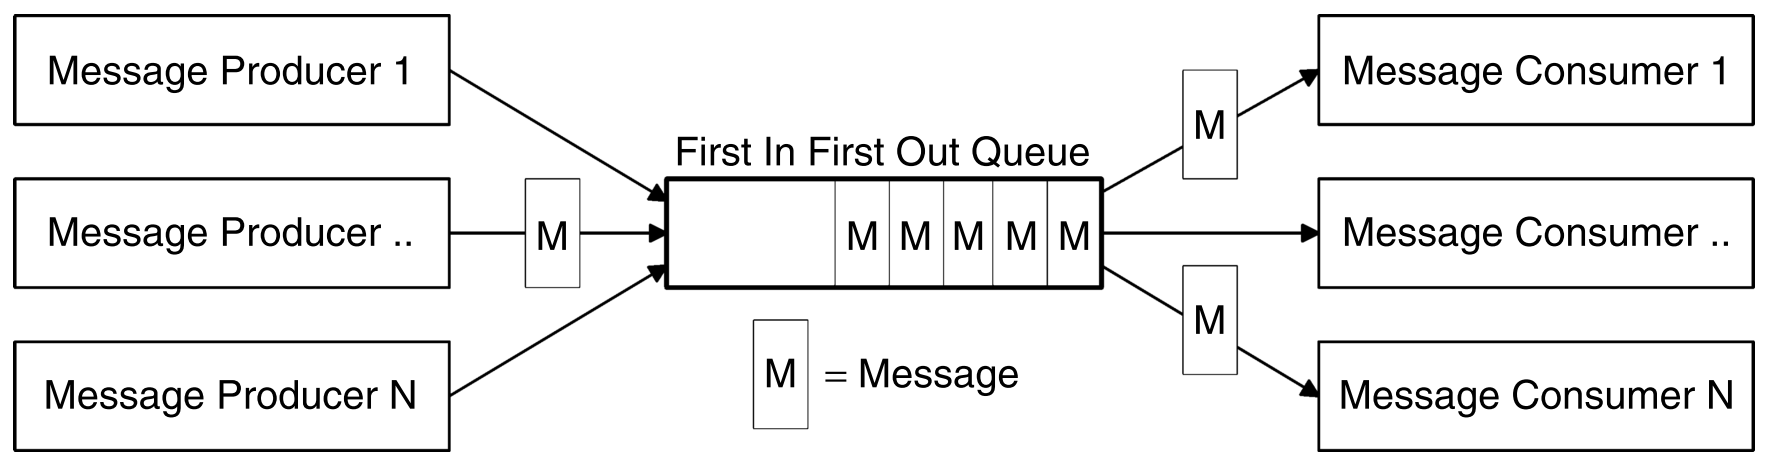
\includegraphics[width=.8\textwidth]{images/middleware_queue.png}
    \caption{A Senerio where Queue is used in Message-Oriented Middleware\cite{CurryMfc2004}}
    \label{fig:diagram}
\end{figure}

Both \emph{components} and \emph{connectors} (or \emph{channels}) are well-known concepts in component-based software engineering. Though having different names, their semantics all turn out to the same nature, \emph{automata}. Following with the idea, we introduce a compositional block named \emph{system}, where automata can be declared as either components or connections. The abstract syntax tree of systems is shown as follows.
\begin{bnf}
    \ntsym{system} ::= & \tsym{system} \ntsym{template}^?\ntsym{identifier} \tsym{(} \ntsym{port}^* \tsym{)} \tsym{\{}\\
    & (\tsym{internals} \ntsym{identifier}^+)^? \\
    & (\tsym{components} \tsym{\{} \ntsym{componentDecl}^* \tsym{\}})^? \\
    & \tsym{connections} \tsym{\{} \ntsym{connectionDecl}^* \tsym{\}} \tsym{\}}\\
    \ntsym{componentDecl} ::= & \ntsym{identifier}^+ \tsym{:} \ntsym{systemType} \\
    \ntsym{connectionDecl} ::= & \ntsym{systemType} \ntsym{params} \tsym{(} \ntsym{portName}^+ \tsym{)}
\end{bnf}

The interface of a system (i.e. its template, name, and ports) shares exactly the same form and meaning with interfaces of automata, which also implies that system is NOT a special semantics unit, but simply an compositional approach to pile up automata. A system is composed of internal nodes (optional), components(optional) and a set of connections.

\smalltitle{Components} Automata can be declared as components in a system. Ports of a component can be referred simply by \texttt{component.portname} where \emph{portname} is the identifier used in its declaration. 

\smalltitle{Connections} Connections, e.g. the arrows in Figure. \ref{fig:diagram}, are used to connect the ports of components.
Both components and connections are supposed to execute concurrently as automata.

\smalltitle{Internals} Directly connecting one port to another is far from enough when modeling complicated systems. For example, in Figure. \ref{fig:diagram} queue work as a connection between consumers and producers. However, since connections to the middleware are dynamically established or disconnected, we still need an extra merger (from producers to the queue) and an extra replicator (from the queue to the consumers) to achieve our goal. When defining internal nodes, we don't have to specify their types. They should be automatically solved by \lang{}.

\begin{example}[\lang{} Model of the System in Figure. \ref{fig:diagram}] In the previous figure, a simple scenario is presented where a queue is used as a message-oriented middleware. To model this scenario, we need two automata \emph{Producer} and \emph{Consumer} (definitions are omitted due to space limit) that produce or consume message of type \emph{T}.
\begin{lstlisting}
automaton <T:type> Producer (OUT: out T) { ... }
automaton <T:type> Consumer (IN: in T) { ... }

system <T:type> middleware_in_use () {
    components {
        producer_1, producer_2, producer_3 : Producer<T>;
        consumer_1, consumer_2, consumer_3 : Consumer<T>;
    }
    internals { M1, M2 }
    connections {
        Merger<T>(producer_1.OUT, producer_2.OUT, producer_3.OUT, M1);
        Queue<T>(M1, M2);
        Replicator<T>(M2, consumer_1.IN, consumer_2.IN, consumer_3.IN);
    }
}
\end{lstlisting}
\end{example}

Since the example is rather trivial, all the connections and components are automata here. But since automata and systems share the same form of interface, it's also valid to use systems as connections or components.

\label{subsec:functions}
% \section{Syntax of \lang{}}
\label{sec:syntax}

In this section, we introduce the syntax of \lang{}, \liyi{represented by a variant of Extended Backus-Naur Form (known as EBNF) where:}
\begin{itemize}
    \item \liyi{Terminal symbols are written in \tsym{monospaced fonts}.}
    \item \liyi{Non-terminal productions are encapsulated in $\ntsym{angle brackets}$}.
    \item \liyi{We use question marks ($^?$) to denote ``zero or one occurence'', star symbol ($^*$) to denote ``zero or more occurence'' and plus sign ($^+$) to denote ``one or more occurence''.}
\end{itemize}

A \lang{} \emph{program} is defined as follows.
\begin{bnf}
    \ntsym{program} ::=  (& \ntsym{typedef} | \ntsym{function} | \ntsym{automaton} | \ntsym{system})^*
\end{bnf}

\liyi{
\emph{Typedef}s specifying alias for given types.
\emph{Function}s defining customized functions.
\emph{System}s declaring hierarchical structures of components and connections between them. Both components and connections are described by automata.
}

\subsection{Type System}
\label{subsec:typesystem}
\lang{} provides a rich-featured type system that supports various data types that are widely used in both formal modeling languages and programming languages.

\smalltitle{Primitive Types} Table \ref{table:primitivetypes} shows the primitive types supported by \lang{} including: \emph{ integers and bounded integers,  real numbers with arbitrary precision, boolean values, single characters (ASCII only) and finite enumerations}.

\begin{table}
    \caption{Primitive Data Types}
    \label{table:primitivetypes}
    \centering
    \begin{tabular}{lcr}
        \hline
        Name & Declaration & Term Example \T\B \\
        \hline
        \T 
        Integer & \texttt{int} & \texttt{-1,0,1} \\
        Bounded Integer\hspace{0.5cm} & \texttt{int lowerBound .. upperBound}\hspace{0.5cm} & \texttt{-1,0,1} \\
        Real & \texttt{real} & \texttt{0.1, 1E-3} \\
        Boolean & \texttt{bool} & \texttt{true, false} \\
        Character & \texttt{char} & \texttt{'a', 'b'} \\
        \B Enumeration & \texttt{enum {item$_1$, ..., item$_n$}} & \texttt{enumname.item} \\
        \hline
    \end{tabular}
\end{table}

\noindent\emph{Composite Types.} Composite types can be used to construct complex data types from simpler ones. Several composite patterns are introduced as follows:

\begin{table}
    \caption{Composite Data Types (\texttt{T} denotes an arbitrary data type)}
    \centering
    \begin{tabular}{lr}
        \hline
        Name & Declaration \T\B \\
        \hline
        \T Tuple  & \texttt{T$_1$,...,T$_n$ }\\
        Union & \texttt{T$_1$|...|T$_n$ } \\
        Array & \texttt{T [length]}\\
        List & \texttt{T []} \\
        Map & \texttt{map [T$_{key}$] T$_{value}$} \\
        Struct\hspace{1cm} & \texttt{struct \{ field$_1$:T$_1$,..., field$_n$:T$_n$ \}} \\
        \B Initialized & \texttt{T$_{base}$ init term} \\
        \hline
    \end{tabular}
\end{table}

\begin{itemize}
    \item \emph{Tuple}. The \emph{tuple} operator `,' can be used to construct a finite tuple type with several base types.
    \item \emph{Union}. The \emph{union} operator `$|$' is designed to combine different types as a more complicated one. 
    \item \emph{Array} and \emph{List}. An \emph{array} $T[n]$ is a finite ordered collection containing exactly $n$ elements of type $T$. Moreover, a \emph{list} is an array of which the capacity is not specified, i.e. list is a dynamic array.
    \item \emph{Map}. A \emph{map }[$T_{key}$] $T_{val}$ is a dictionary that maps a key of type $T_{key}$ to a value of type $T_{val}$.
    \item \emph{Struct}. A \emph{struct }\{$field_1:T_1,\cdots,field_n:T_n$\} contains a finite number of fields, each has  a unique identifier $field_i$ and a particular type $T_i$.
    \item \emph{Initialized}. An initialized type is used to specify default value of a type $T_{base}$ with \texttt{term}.
\end{itemize}

\noindent\emph{Parameter Types}. A generalizable automaton or system that includes a template function or template component needs to be defined on many occasions. For example, a binary operator that supports various operations ($+$,$\times$, etc.), or an encrypted communication system that supports different encryption algorithms. Parameter types make it possible to take functions, automata or systems as template parameters. \lang{} supports two parameter types: 
\begin{enumerate}
    \item \emph{An Interface}, denoted by \texttt{interface (port$_1$:T$_1$,$\cdots,$port$_n$:T$_n$)}, defines a parameter that could be any \emph{automaton} or \emph{system} with exactly the same interface (i.e. number, types and directions of the ports are a perfect match). Interfaces are only used in templates of \emph{system}s.
    % TODO: interfaces are not permitted in automata since automata do not support hierarchical structure
    \item \emph{A Function}, denoted by \texttt{func (arg$_1$:T$_1$,$\cdots, $arg$_n$:T$_n$):T}, defines a function that has the argument types $\texttt{T}_1,\cdots,\texttt{T}_n$ and result types \texttt{T}. Functions are permitted to appear in templates of \emph{other functions}, \emph{automata} and \emph{system}s.
\end{enumerate}

For simplicity, we use $Dom(T)$ to denote the value domain of type $T$, i.e. the set of all possible value of $T$.

\begin{example}[Types Used in a Queue] A queue is a well-known data structure being used in various message-oriented middlewares. In this example, we introduce some type declarations and local variables used in an automaton \texttt{Queue} defining the queue structure. As shown in the following code fragment, we declare a singleton enumeration \texttt{NULL}, which contains only one element \texttt{null}. The buffer of a queue is in turn formalized as an array of \texttt{T} or \texttt{NULL}, indicating that the elements in the queue can be either an assigned item or empty. The head and tail pointers are defined as two bounded integers.
\begin{lstlisting}[basicstyle=\scriptsize\ttfamily]
typedef enum {null} init null as NULL;
automaton <T:type,size:int> Queue(A:in T, B:out T) {
    variables {
        buf : ((T | NULL) init null) [size];
        phead, ptail : int 0 .. (size - 1) init 0;
    }
    ...
}
\end{lstlisting}
\label{exp:typeinqueue}
\end{example}

\subsection{Functions}
\label{subsec:functions}

Functions are used to encapsulate and reuse complex computation processes. In \lang{}, the notion of \emph{functions} is a bit different from most existing programming languages. \lang{} functions include no control statements at all but assignments, and have access only to its local variables and arguments. This design makes functions' behavior more predictable. In fact, the behavior of functions in \lang{} can be simplified into mathematical functions. 

The abstract syntax tree of functions is as follows.

\begin{bnf}
    \ntsym{funcDecl} ::= & \tsym{function} \ntsym{template}^? \ntsym{identifier} \ntsym{funcInterface} \tsym{\{} \\
    & (\tsym{variables} \tsym{\{} \ntsym{varDecl}^* \tsym{\}})^? \\
    & \tsym{statements} \tsym{\{} \ntsym{assignStmt}^* \ntsym{returnStmt} \tsym{\}} \\
    \ntsym{funcInterface} ::= & \liyi{\tsym{(} (\ntsym{identifier} \tsym{:} \ntsym{type})^* \tsym{)} \tsym{:} \ntsym{type}}\\
    \ntsym{assignStmt} ::= & \liyi{\ntsym{term} (\tsym{,} \ntsym{term})^* \tsym{:=} \ntsym{term} (\tsym{,} \ntsym{term})^*} \\
    \ntsym{returnStmt} ::= & \tsym{return} \ntsym{term} \\
    \ntsym{varDecl} ::= & \ntsym{identifier} \tsym{:} \ntsym{type} (\tsym{init} \ntsym{term})^? 
\end{bnf}
Basically, a function definition includes the following parts.

\smalltitle{Template} A function may contain an optional template with a set of parameters. A parameter can be either a \emph{type} parameter (decorated by \texttt{type}) or a \emph{value} parameter (decorated by its type). Values of the parameters should be clearly specified during compilation. Once a parameter is declared, it can be referred in all the following language elements, e.g. parameter declarations, arguments, return types and statements.

\smalltitle{Name} An identifier that indicates the name of this function.

\smalltitle{Type} Type of a function is determined by the \emph{number and types of arguments}, together with \emph{the type of its return value.} 

\smalltitle{Body} Body of a function includes an optional set of local variables and a list of ordered \liyi{(assignment or return) statements. In an assignment statement, local variables, parameters and arguments can be referenced, but only local variables are writable.} The list of statements always ends up with a \texttt{return} statement.

\begin{example}[Incline Operation on Queue Pointers] Incline operation of pointers are widely used in a \emph{round-robin} queue, where storage are reused circularly. The \texttt{next} function shows how pointers in such queues (denoted by a bounded integer) are inclined. 
    \label{exp:successor_function}
    \begin{lstlisting}
function <size:int> next(pcurr:int 0..(size-1)) : int 0..(size-1) {
    statements { return (pcurr + 1) % size; }
}
    \end{lstlisting}
\end{example}

\subsection{Automaton : The Basic Behavioral Unit}

Automata theory is widely used in formal verification, and its variations, finite-state machines for example, are also accepted by modeling tools like NI LabVIEW and Mathworks Simulink/Stateflow.

Here we introduce the notion of \emph{automaton} as the basic behavior unit. Compared with other variations, an \emph{automaton} in \lang{} contains local variables and typed ports that support complicated behavior and powerful communication. The abstract syntax tree of \emph{automaton} is as follows.

\begin{bnf}
    \ntsym{automaton} ::=& \tsym{automaton}\ntsym{template}^?\ntsym{identifier} \tsym{(} \ntsym{port}^* \tsym{)} \tsym{\{}\\
    & (\tsym{variables} \tsym{\{} \ntsym{varDecl}^* \tsym{\}})^? \\
    & \tsym{transitions} \tsym{\{} \ntsym{transition}^* \tsym{\}} \tsym{\}} \\
    \ntsym{port} ::=& \ntsym{identifier} \tsym{:} (\tsym{in}|\tsym{out}) \ntsym{type} \\
    \ntsym{transition} ::=& \ntsym{guardedStmt} | \tsym{group} \tsym{\{} \ntsym{guardedStmt}^* \tsym{\}}\\
    \ntsym{guardedStmt} ::=& \ntsym{term} \tsym{->} (\ntsym{stmt} | \tsym{\{} \ntsym{stmt}^* \tsym{\}}) \\
    \ntsym{stmt} ::=& \liyi{\ntsym{assignStmt}} | \tsym{sync} \ntsym{identifier}^+
\end{bnf}

\smalltitle{Template} Compared with templates in functions, templates in automata provide support for parameters of \emph{function type}.

\smalltitle{Name} The identifier of an automaton.

\smalltitle{Type} Type of an automaton is determined by the \emph{number} and \emph{type}s of its ports. Type of a port contains its \emph{direction} (either \texttt{in} or \texttt{out}) and its \emph{data type}. For example, a port $P$ that takes integer values as input is denoted by \texttt{P:in int}. To ensure the well-definedness of automata, ports are required to have an \emph{initialized} data type, e.g. \texttt{int 0..1 init 0} instead of \texttt{int 0..1}.

\smalltitle{Variables} Two classes of variables are used in an automaton definition. \emph{Local variables} are declared in the \emph{variables} segment, which can be referenced only in its owner automaton. \liyi{\emph{Port variables}, on the other hand, are shared variables that describe the status and value of ports.}

\liyi{Port variables are denoted as fields of ports.}
An arbitrary port $P$ has two corresponding Boolean port variables \texttt{P.reqRead} and \texttt{P.reqWrite} indicating whether there is any pending \emph{read} or \emph{write} requests on $P$, and a data field \texttt{P.value} indicating the current value of $P$. \liyi{When automata are combined, port variables are shared between automata to perform communications. To avoid data-conflict, we require that only \texttt{reqRead} and \texttt{value} fields of input ports, and \texttt{reqWrite} fields of output ports are writable. Informally, an automaton only requires data from its input port and writes data to its output port.}

\smalltitle{Transitions}
In \lang{}, behavior of an automaton is described by a \liyi{list} of guarded transitions (groups).
% , with no explicit concept of locations (actually locations can be easily encoded as local enumeration variables).
A \emph{transition} (denoted by \emph{guard} \texttt{->} \emph{statements}) comprises two parts, a Boolean term \emph{guard} that declares the activating condition of this transition, and a (sequence of) statement(s) describing how variables are updated when the transition is fired.

We have two types of statements supported in automata:
\begin{itemize}
    \item \emph{Assignment Statement} (\texttt{var$_1$,...,var$_n$ := term$_1$,...,term$_n$}). Assignment statements update variables with new values where only local variables and writable port variables are assignable.
    \item \emph{Synchronizing Statement} (\texttt{sync port$_1$,...,port$_n$}). Synchronizing statements are used as synchronizing \emph{flag}s when joining multiple automata. In a synchronizing statement, the order of ports being synchronized is arbitrary. For further details, please refer to Section \ref{subsec:composition}.
\end{itemize}

% Synchronizing statements are also important flags to distinguish between external transitions and internal transitions.
\liyi{A transition is called \emph{external} iff. it synchronizes with its environment through certain ports or \emph{internal} nodes with synchronizing statements. In such transitions, we require that \emph{any assignment statements including reference to an input(output) port should be placed after(before) its corresponding synchronizing statement}}.

We use $g\rightarrow S$ to denote a transition, where $g$ is the guard formula and $S=[s_1,\cdots,s_n]$ is a sequence of statements. 

Transitions in \lang{} automata are \liyi{literally ordered}. \liyi{Given a list of transitions $g_1\rightarrow S_1,\cdots, g_n\rightarrow S_n$ where $\{g_{i_j}\}_{j=1,\cdots,m}$ is satisfied, only the transition $g_{min\{i_j\}}\rightarrow S_{min\{i_j\}}$ will be fired. In other words, $g_i\rightarrow S_i$ is fired iff. $g_i$ is satisfied and for all $0<j<i$, $g_j$ is unsatisfied.}
% Formally speaking, suppose $g_1\rightarrow S_1,\cdots,g_n\rightarrow S_n$ is a list of transitions with priority, we could use an equivalent form to rewrite them as the followings, where priority is not necessary any more.
% \[
%     g_1\rightarrow S_1, \lnot g_1\land g_2\rightarrow S_2,\cdots,\lnot g_1\land \lnot g_2\land\cdots\land \lnot g_{n-1} \land g_n\rightarrow S_n
% \]

\begin{example}[Transitions in Queue] For a queue, we use internal transitions to capture the modifications corresponding to the changes of its environment. For example, the automaton \texttt{Queue}  tries to:
\begin{enumerate}
    \item Read data from its input port $A$ by setting \texttt{A.reqRead} to \emph{true} when the buffer isn't full.
    \item Write the earliest existing buffered data to its output port $B$ when the buffer is not empty. 
\end{enumerate}
External transitions, on the other hand, mainly show the implementation details for the enqueue and dequeue operations.
\begin{lstlisting}[basicstyle=\scriptsize\ttfamily]
// internal transitions
!A.reqRead && (buf[phead] == null) -> A.reqRead := true;
A.reqRead && (buf[phead] != null) -> A.reqRead := false;
!B.reqWrite && (buf[ptail] != null) -> B.reqWrite := true;
B.reqWrite && (buf[ptail] == null) -> B.reqWrite := false;

// enqueue operation (as an external transition)
(A.reqRead && A.reqWrite) -> {
    sync A; // read data from input port A
    buf[phead] := A.value; phead := next(phead);
}
// dequeue operation (as an external transition)
(B.reqRead && B.reqWrite) -> {
    B.value := buf[ptail]; ptail := next(ptail);
    sync B; // write data to output port B
}
\end{lstlisting}
\label{exp:trans_queue}
\end{example}

If all transitions are organzied with priority, the automata would be fully deterministic. However, in some cases non-determinism is still more than necessary. Consequently, we introduce the notion of \emph{transition group} to capture non-deterministic behavior. A transition group $t_G$ is formalized as a finite set of guarded transitions
$t_G=\{t_1,\cdots, t_n\}$ where $t_i=g_i\rightarrow S_i$ is a single transition with guard $g_i$ and a sequence of statements $S_i$.

Transitions encapsulated in a \texttt{group} are not ruled by priority. Instead, the group itself is literally ordered w.r.t. other groups and single transitions (basically, we can take all single transitions as a singleton transition group).

\begin{example}[Another Queue Implementation] In Example \ref{exp:trans_queue}, when both \emph{enqueue} and \emph{dequeue} operations are activated, \emph{enqueue} will always be fired first. Such a queue may get stuff up immediately when requests start accumulating, and in turn lead to excessive memory usage. With the help of transition groups, here we show another non-deterministic implementation which solves this problem.
\begin{lstlisting}
group {
    (A.reqRead && A.reqWrite) -> {
        sync A; buf[phead] := A.value; phead := next(phead);
    }
    (B.reqRead && B.reqWrite) -> {
        B.value := buf[ptail]; ptail := next(ptail); sync B;
    }
}
\end{lstlisting}
In the above code fragment, the two external transitions are encapsulated together as a transition group. Consequently, firing of the dequeue operation doesn't rely on deactivation of the enqueue operation.
\label{exp:transgroup_queue}
\end{example}


We use a 3-tuple $A=\langle Ports, Vars, Trans_G \rangle$ to represent an automaton in \lang{}, where $Ports$ is a set of ports, $Vars$ is a set of local variables (the set of port variables are denoted by $Adj(A)$, which can be obtained from $Ports$ directly) and $Trans_G=[t_{G_1},\cdots,t_{G_n}]$ is a sequence of transition groups, where all single transitions are encapsulated as singleton transition groups.

\subsection{System : The Composition Approach}
\label{subsec:system}

Theoretically, automata and their product is capable to model various classical applications. However, modeling complex systems through a mess of transitions and tons of local variables could become a real disaster.

As mentioned before, \lang{} is designed to help the programmers, even nonprofessionals, to enjoy the convenience of formal tools\liyi{, which} is exactly the reason why we introduce the notion of \emph{system} \liyi{as an \emph{encapsulation mechanism}}. Basically, a \emph{system} is the textual representation of a hierarchical diagram where automata and smaller systems are organized as \emph{component}s or 
\emph{connection}s. 

% Hierarchical diagrams have already been used in various modeling tools (for example, SCADE \cite{AbdullaISoLA2006,BerryScp1992}, Simulink \cite{hahn2016essentialsimulink} and LabVIEW \cite{labview}). However, in most tools, connections are simply synchronous link that seal two ports together. Inspired by the connectors in Reo, \lang{} to declare an automaton as a connection, which lead to more powerful and intuitive diagrams. 

\begin{example}[A Message-Oriented Middleware]
    A simple diagram of a message-oriented middleware \cite{CurryMfc2004} is provided in Fig. \ref{fig:diagram}, where a queue works as a connector to coordinate the message producers and consumers.
\end{example}

\begin{figure}
    \centering
    \tikzstyle{component}=[
    rectangle,
    rounded corners,
    double,
    double distance = 1pt,
    draw
]

\begin{tikzpicture}[remember picture]
    \node[component] (producer1) at (-3,0.8) {Producer 1};
    \node[component] (producer2) at (-3,0) {Producer 2};
    \node[component] (producer3) at (-3,-0.8) {Producer 3};

    \mixednode{(A1)}{(-1,0)};
    \mixednode{(B1)}{(1,0)};

    \draw [->] (-1.5,0) to (A1);
    \draw [-] (1.5,0) to (B1);

    \fifoe{(A1)}{(B1)}{node [above=5,xshift=1] {Queue}}

    \node[component] (consumer1) at (3,0.8) {Consumer 1};
    \node[component] (consumer2) at (3,0) {Consumer 2};
    \node[component] (consumer3) at (3,-0.8) {Consumer 3};

    \draw [-] (producer1) to [out=0,in=180] (-1.5,0);
    \draw [-] (producer2) to (-1.5,0);
    \draw [-] (producer3) to [out=0,in=180] (-1.5,0);

    \draw [->] (1.5,0) to [out=0,in=180] (consumer1);
    \draw [->] (1.5,0) to [out=0,in=180] (consumer2);
    \draw [->] (1.5,0) to [out=0,in=180] (consumer3);

\end{tikzpicture}
    \caption{A Scenario where Queue is used as Message-Oriented Middleware}
    \label{fig:diagram}
\end{figure}

% \begin{figure}
%     \centering
%     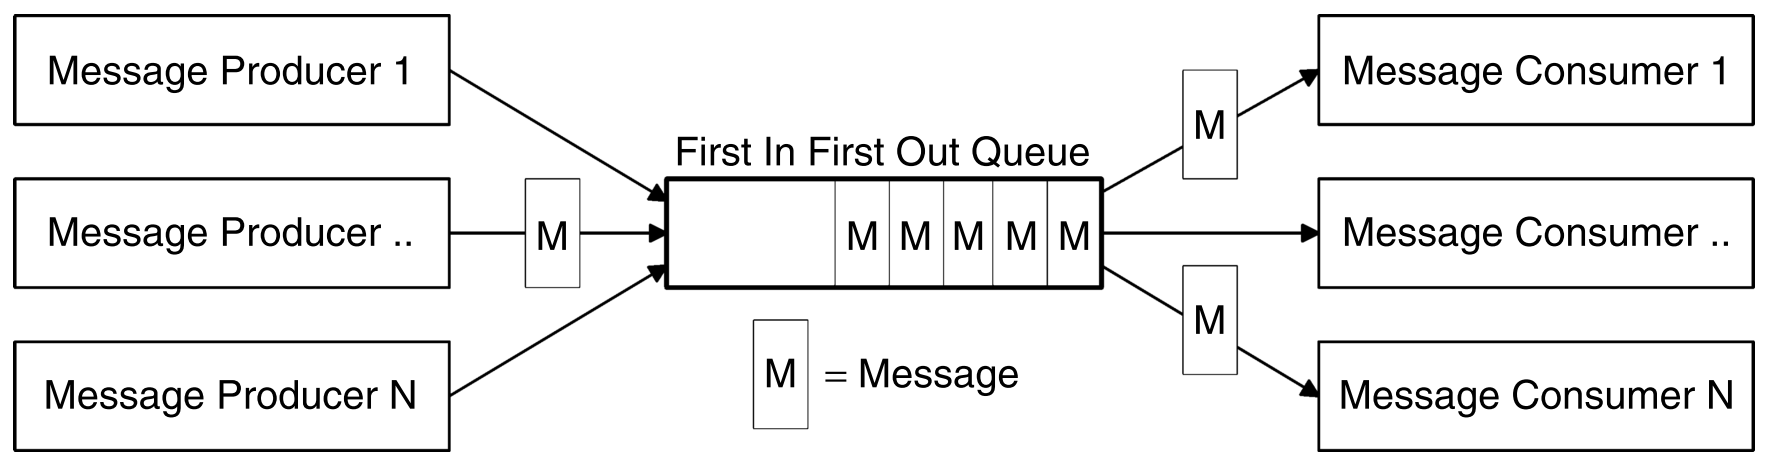
\includegraphics[width=.8\textwidth]{images/middleware_queue.png}
%     \caption{A Scenario where Queue is used as Message-Oriented Middleware}
%     \label{fig:diagram}
% \end{figure}

The abstract syntax tree of \emph{system}s is as follows:
\begin{bnf}
    \ntsym{system} ::= & \tsym{system} \ntsym{template}^?\ntsym{identifier} \tsym{(} \ntsym{port}^* \tsym{)} \tsym{\{}\\
    & (\tsym{internals} \ntsym{identifier}^+)^? \\
    & (\tsym{components} \tsym{\{} \ntsym{componentDecl}^* \tsym{\}})^? \\
    & \tsym{connections} \tsym{\{} \ntsym{connectionDecl}^* \tsym{\}} \tsym{\}}\\
    \ntsym{componentDecl} ::= & \ntsym{identifier}^+ \tsym{:} \ntsym{systemType} \\
    \ntsym{connectionDecl} ::= & \ntsym{systemType} \ntsym{params} \tsym{(} \ntsym{portName}^+ \tsym{)}
\end{bnf}

% The \emph{type} of a system (i.e. its template, name, and ports) shares exactly the same form and meaning with \emph{type} of an automaton. This also suggests that system is NOT a special semantics unit, but simply an compositional approach to pile up automata.
% We declare a system with its template, name and type, then it is implemented by an optional set of \emph{internal node}s, an optional set of \emph{component}s and a set of \emph{connection}s.

\smalltitle{Template} In templates of systems, all the parameter types being supported include: \emph{a)} parameters of abstract type \texttt{type}, \emph{b)} parameters of primitive types and composite types, and \emph{c)} interfaces and functions.

\smalltitle{Name and Type} Exactly the same as \emph{name} and \emph{type} of an automaton.

\smalltitle{Components} In \texttt{components} segments, we can declare any entity of an \emph{interface type} as components, e.g. an automaton, a system, or a parameter of interface type. 
Ports of a component can be referenced by \texttt{identifier.portName} once declared.

\smalltitle{Connections} Connections, e.g. the queue in Fig. \ref{fig:diagram}, are used to connect \emph{a) the ports of the system itself, b) the ports of its components, and c) the internal nodes}. We declare the connections in \texttt{connections} segments.
Both components and connections are supposed to run as automata in parallel.

\smalltitle{Internals} \liyi{Sometimes we need to combine multiple connections to perform more complex coordination behavior. Internal nodes, declared in \texttt{internals} segments, are untyped identifiers which are capable to weld two ports with consistent data-flow direction. For example, in Fig.~\ref{fig:diagram} the two internal nodes (denoted by $\bullet$) are used to combine a \emph{replicator}, a queue and a \emph{merger} together to work as a multi-in-multi-out queue.}


% Essentially, data flow in an internal node should always follow the same direction, i.e. an internal node doesn't collect or generate any data, it only receives from one end and forward it simultaneously. The direction, together with the type of an internal node, should be determined when being compiled.

A system is denoted by a 4-tuple
$S=\langle Ports, Entities, Internals, Links\rangle$ where $Ports$ is a set of ports, $Entities$ is a set of automata or systems (including both components and connections), $Internals$ is a set of internal nodes and $Links$ is a set of pairs, where each element of such a pair is either a port or an internal node. A link $\langle p_1,p_2\rangle$ suggests that $p_1$ and $p_2$ are linked together. A well-defined system satisfies the following assumptions:

% TODO:
\begin{enumerate}
    \item $\forall \langle p_1,p_2\rangle \in Links$, data transfer from $p_1$ to $p_2$. For example, if $p_1\in Ports$ is an input port, $p_2$ could be
    \begin{itemize}
        \item an output port of the system ($p_2\in Ports$), 
        \item an input port of some automaton $A_i\in Automata$ ($p_2\in A_i.Ports$), or
        \item an internal node ($p_2\in Internals$).
    \end{itemize}
    \item $\forall n\in Internals,\exists!p_1,p_2$, s.t. $\langle p_1,n\rangle ,\langle n,p_2\rangle\in Links$ and $p_1,p_2$ have the same data type.
\end{enumerate}

\begin{example}[\lang{} Model of the System in Fig. \ref{fig:diagram}] In Fig. \ref{fig:diagram}, a simple scenario is presented where a queue is used as a message-oriented middleware. To model this scenario, we need two automata \emph{Producer} and \emph{Consumer} (details are omitted due to space limit, and can be found at \cite{medmodels}) that produce or consume messages of type \emph{T}.
\begin{lstlisting}
automaton <T:type> Producer (OUT: out T) { ... }
automaton <T:type> Consumer (IN: in T) { ... }

system <T:type> middleware_in_use () {
    components {
        producer_1, producer_2, producer_3 : Producer<T>;
        consumer_1, consumer_2, consumer_3 : Consumer<T>;
    }
    internals  M1, M2 ;
    connections {
        Merger<T>(producer_1.OUT, producer_2.OUT, producer_3.OUT, M1);
        Queue<T>(M1, M2);
        Replicator<T>(M2, consumer_1.IN, consumer_2.IN, consumer_3.IN);
    }
}
\end{lstlisting}
\label{exp:middleware_system}
\end{example}

\section{Semantics}
\label{sec:semantics}

\subsection{Configurations of Automata}
\label{subsec:config}
% TODO: formalization of adjoint variables
Configurations are used to represent the state of an automaton. Since we don't have locations here, it only depends on the values of its locally accessible variables, which includes both \emph{adjoint variables} and \emph{local variables}.

\begin{definition}[Valuation]
An evaluation of a set of variables $Vars$ is defined as a function $v$ that satisfies $\forall x\in Vars,v(x)\in Dom(type(x))$. We denote all the possible evaluations of a variable set $Vars$ as $Val(Vars)$.
% TODO: how to say `without confusion`
\end{definition}

\begin{definition}[Configuration] A configuration of an automaton $A=\langle Ports,$ $Vars,Trans_G\rangle$ is defined as a tuple $(v_{loc},v_{adj})$ where $v_{loc}\in Val(Vars)$ is a valuation on local variables, and $v_{adj}\in Val(Adj(P))$ is a valuation on adjoint variables. 
\end{definition}

\subsection{Canonical Form of Transitions}
\label{subsec:canonical}

% TODO: what features?
% As mentioned before, transitions in an automaton have fantastic features to write simple but powerful models, including \emph{a) Priority}. In this subsection we introduce how these features work, and how to convert the rich-featured models to traditional ones.
\begin{definition}[Canonical Transitions]
A transition $t=g\rightarrow\{s_1,\cdots,s_n\}$ is canonical iff. its statements $\{s_i\}$ is an interleaving sequence of assignments and performs which start from an assignment, e.g. \texttt{a:= exp$_1$; perform A; b:= exp$_2$; $\cdots$}.
\end{definition}
We only need to simple steps to canonicalize a transition, they are:
\begin{enumerate}
    \item Merging the contiguous assignments. As mentioned before, an assignment statement is represented as a function $f:EV\rightarrow EV$. Thus a list of multiple assignments $f_1,\cdots, f_n$ can be simplified by $f=f_1\circ\cdots \circ f_n$.
    \item Any two adjacent performs should be separated by a identical assignment $id_{EV}$. 
\end{enumerate}

\smalltitle{Observable} A transition is always \emph{observable}, i.e. it will makes some difference to the context. For example, without this assumption, a transition \texttt{true -> x := x} will block the whole model by endless meaningless executions.

\begin{definition}[Canonical Transition Groups]
    A transition group is canonical iff. it only contains one canonical transition.
\end{definition}

\smalltitle{Priority} Given a set of ordered transitions.
\[
    \{g_1\rightarrow S_1,g_2\rightarrow S_2,\cdots,g_n\rightarrow S_n\}
\]
As required by the \emph{priority} assumption, a transition can be fired only if all the previous ones are not enabled (i.e. their guards are not satisfied) yet. In \lang{}, this feature is resolved simply by adding $\lnot g_i$ to all $g_j(j>i)$. E.g.
\[
    \{g_1\rightarrow S_1, g_2\land(\lnot g_1)\rightarrow S_2,\cdots,g_n\land(\lnot g_1\land \lnot g_2\land\cdots\land \lnot g_{n-1})\rightarrow S_n\}
\]
Now let's consider a set of ordered groups $t_{G_i}$, where $t_{G_i}$ contains $l_i$ transitions,
\begin{small}
\[
    T_G=\{t_{G_1}=\{g_{11}\rightarrow S_{11},\cdots, g_{1l_1}\rightarrow S_{1l_1}\},\cdots,t_{G_n}=\{g_{n1}\rightarrow S_{n1},\cdots,g_{nl_n}\rightarrow S_{nl_n}\}\}
\]
\end{small}
Informally speaking, once a transition in $t_{G_1}$ is enabled, all the other transitions in $t{G_i}(i>1)$ should be strictly prohibited from being fired. We use $enab(t_G)$ to denote the condition where at least one transition in $t_G$ is enabled, formalized as
\[
    enab(t_G=\{g_1\rightarrow S_1,\cdots, g_n\rightarrow S_n\}) = g_1\lor\cdots\lor g_n
\]
Then we can generate the new set of transitions with no dependency on priority:
\begin{eqnarray*}
    g_{11}\rightarrow S_{11},&\cdots&,g_{1l_1}\rightarrow S_{1l_1}, \\
    g_{21}\land \lnot enab(t_{G_1})\rightarrow S_{21}, &\cdots&, g_{2l_2} \land \lnot enab(t_{G_1})\rightarrow S_{2l_2}, \cdots \\
    g_{n1}\land \lnot enab(t_{G_1},\cdots,t_{G_{n-1}})\rightarrow S_{n1}, &\cdots&, g_{nl_n} \land \lnot enab(t_{G_1},\cdots,t_{G_{n-1}})\rightarrow S_{nl_n} \\
\end{eqnarray*}
where $enab(t_{G_1},\cdots,t_{G_{n-1}})$ is an abbreviation of $enab(t_{G_1})\lor\cdots\lor enab(t_{G_{n-1}})$. It indicates that at least one group in $t_{G_i}$ is enabled.
\subsection{From System to Automaton}
\label{subsec:composition}

Systems, as shown previously, are simply introduced to construct automata in a more natural way. Now we show how such a system can be flatten as a standard automaton.

% TODO: canonical form of a transition mus requires a interleaving form, may be filled
% with non-sense assignments
% TODO: topological sorting
\begin{algorithm}[H]
    \caption{Scheduling in a Synchronous Set of External Transitions}
    \label{alg:synchronize}
    \begin{algorithmic}[1]
        \REQUIRE $t_1,t_2,\cdots,t_n$ are transitions (canonical form)
        \ENSURE $t=\mbox{\texttt{Schedule}}(t_1,\cdots,t_n)$
        \IF{$\{t_i\}$ don't belong to different automata or $\exists t_i$ is internal}
            \STATE $t\leftarrow null$
            \RETURN
        \ENDIF
        \STATE \emph{t.g, t.S} $\leftarrow \bigwedge_i t_i.g,\:\{\}$
        \FOR{$i\leftarrow 1,\cdots,n$}
            \IF {$t_i.s_1$ is an \emph{assignment}}
            \STATE add $t_i.s_1$ to the head of $t.S$
            \ENDIF
            \STATE $p$ $\leftarrow$ the first \emph{perform} statement
            \WHILE {$p$ $\neq$ \emph{null}}
                \STATE $a\leftarrow$ the \emph{assignment} statement after $p$
                \STATE $p'\leftarrow$ the next \emph{perform} statement after $p$
                \IF {$p\in t.S$}
                    \STATE insert $a$ to $t.S$ exactly after $p$
                    \STATE remove $p$ from $t.S$
                \ENDIF
            \ENDWHILE
        \ENDFOR
        \STATE $t\leftarrow$ \texttt{Canonicalize($t$)}
    \end{algorithmic}
\end{algorithm}

\begin{algorithm}[H]
    \caption{Compose Several Automatons}
    \label{alg:compose}
    \begin{algorithmic}[1]
        \REQUIRE $A_1,A_2,\cdots,A_n$ are automata
        \ENSURE $A=\mbox{\texttt{Compose}}(A_1,\cdots,A_n)$
        \STATE rename local variables in $A_1,\cdots,A_n$ to avoid duplicated names
        \STATE $A \leftarrow $ empty automaton
        \STATE $ext\_trans\leftarrow \{\}$
        \FOR{$i\leftarrow 1,2,\cdots,n$}
            \STATE add all local variables of $A_i$ to $A$
            \STATE add all internal transitions of $A_i$ to $A$
            \STATE add all external transitions of $A_i$ to $ext\_trans$
        \ENDFOR
        \FOR{$set\_trans\leftarrow$ subset of $ext\_trans$}
            \STATE $newedge\leftarrow \mbox{\texttt{Schedule}}(set\_trans)$ 
            \IF{\emph{newedge $\neq$ null}}
                \STATE add \emph{newedge} to $A$
            \ENDIF
        \ENDFOR
    \end{algorithmic}
\end{algorithm}

\subsection{Automaton as Labelled Transition System}

\begin{definition}[Transition System, TS]
    A transition system is a tuple $(S,\rightarrow)$ where $S$ is a set of states and $\rightarrow\subseteq S\times\Sigma\times S$ is a set of transitions. For simplicity reason, we use $s\rightarrow s'$ to denote $(s,s')$ in $\rightarrow$.
\end{definition}

Suppose $A=\langle Ports, Vars, Trans_G\rangle$ is an automaton, its semantics can be captured by a labelled transition system $\langle S_A, \rightarrow_A\rangle$ where
\begin{itemize}
    \item $S_A$ is the set of all configurations of $A$.
    \item $\rightarrow_A\subseteq S_A\times \Sigma_A\times S_A$ is a set of transitions constructed by the following rules.
\end{itemize}

\begin{mathpar}
    \inferrule* [right=R-InputStatus] {p\in P_{in}}{(v_{loc}, v_{adj})\xrightarrow{}_A(v_{loc},v_{adj}[p.reqWrite\mapsto \lnot p.reqWrite])} \\
    \inferrule* [right=R-InputValue] {p\in P_{in}, val\in type(p.value)}{(v_{loc}, v_{adj})\xrightarrow{}_A(v_{loc},v_{adj}[p.value\mapsto val])} \\
    \inferrule* [right=R-OutputStatus] {p\in P_{out}}{(v_{loc}, v_{adj})\xrightarrow{}_A(v_{loc},v_{adj}[p.reqRead\mapsto \lnot p.reqRead])} \\
    \inferrule* [right=R-Internal] {\{g\rightarrow \{s\}\}\in Trans_G\mbox{ is internal}}{(v_{loc}, v_{adj})\xrightarrow{}_A s(v_{loc},v_{adj})} \\
    \inferrule* [right=R-External] {\{g\rightarrow S\}\in Trans_G\mbox{ is external, } \{s_1,\cdots,s_n\}\mbox{ are the assignments in $S$}}{(v_{loc}, v_{adj})\xrightarrow{}_A s_n\circ\cdots\circ s_1(v_{loc},v_{adj})} \\
\end{mathpar}

The first three rules describe the potential change of context, i.e. the adjoint variables. R-InputStatus and R-OutputStatus shows that the reading status of an output port and status of an input port may changed randomly. And R-InputValue shows that the value of an input port may be updated by the context.

The rule R-Internal models the internal transitions in $Trans_G$. As illustrated previously, an internal transition doesn't contains any perform statement. So its canonical form comprises only one assignment $s$. Firing such a transition will simply apply $s$ to the current configuration.

Meanwhile, R-External models the external transitions, where the automaton need to interact with its context. Fortunately, since all the context change are captured by the first three rules, we can simply regard the context as a set of local variables. Consequently, the only difference between an internal transition and an external transitions is that the later may contains multiple assignments.

%TODO: take queue as an example

\section{Discussion}

\section{Case Study}

\section{Conclusion and Future Work}

\bibliographystyle{splncs03}
\bibliography{fm}

\end{document}